\chapter*{Introducción y objetivos}
\addcontentsline{toc}{chapter}{Introducción y objetivos}

%TODO: poner aquí introducción y objetivos

\textcolor{red}{Completar introducción y añadir objetivos}


\begin{comment}
La introducción deberá:
- Contextualizar el trabajo explicando antecedentes importantes para el desarrollo realizado y efectuando, en su caso, un estudio de los progresos recientes.
- Describir el problema abordado, de forma que el lector tenga desde este momento una idea clara de la cuestión a resolver o del producto  a desarrollar y una  visión general de la solución alcanzada.
- Exponer con claridad las técnicas y áreas matemáticas, así como los conceptos y herramientas de la ingeniería informática que se han empleado.
- Sintetizar el contenido de la memoria.
- Citar las principales fuentes consultadas.

Objetivos del trabajo:
- En  este apartado deberán aparecer con claridad los objetivos inicialmente previstos en la propuesta de TFG y los finalmente alcanzados con indicación de  dificultades, cambios y mejoras respecto a la propuesta inicial. Si procede, es conveniente apuntar de manera precisalas interdependencias entre los distintos objetivos y conectarlos con los diferentes apartados de la memoria. 
Se pueden destacar aquí los aspectos formativos previos más utilizados.
\end{comment}


%\textcolor{red}{Comentario del tutor:}
%\textcolor{red}{Esto es verdad. Pero en algunas ocasiones se nombre a Hamming como el "padre" de la teoría de códigos y a Shannon como el "padre" de la teoría de la información (algo más general). Esto es así porque en el artículo de Shannon se pone como ejemplo cómo corrige un código de Hamming, y Shannon mismo dice que es una construcción de Richard Hamming (creo que se publica después, en 1950). También Golay tiene una nota sobre el tema en 1949. Busca el artículo de Hamming y verás algo más parecido a lo que tratamos aquí. Además, si te lees bien los artículos de Shannon y Hamming te será fácil escribir una introducción para este capítulo, o para la memoria.}

\spacedlowsmallcaps{Contexto}

El inicio de la teoría de información surgió a partir de la publicación de Claude Shannon sobre ``Una teoría matemática sobre la comunicación"\ en 1948 \cite{Shannon_1948}. En este artículo, Shannon explica que es posible transmitir mensajes fiables en un canal de comunicación que puede corromper la información enviada a través de él siempre y cuando no se supere la capacidad de dicho canal. En dicho artículo pone como ejemplo la corrección de un código de Hamming, una construcción de Richard Hamming. Dos años más tarde, Hamming publica ``Error Detecting and Error Correcting Codes"\ \cite{Hamming_1950} y con dicha publicación aparece el inicio de la teoría de códigos. La motivación de este artículo surgió a partir de la preocupación sobre los errores producidos en los ordenadores al operar con grandes números. Es por esto que Hamming expone la importancia de detectar y corregir los errores que se puedan producir y, además, propone algunas soluciones.

Con la teoría de códigos, podemos codificar datos antes de transmitirlos de tal forma que los datos alterados puedan ser decodificados al grado de precisión especificado. Así, el principal problema es determinar el mensaje que fue enviado a partir del recibido. El Teorema de Shannon nos garantiza que el mensaje recibido coincidirá con el que fue enviado un cierto porcentaje de las veces. Esto hace que el objetivo de la teoría de códigos sea crear códigos que cumplan las condiciones de este teorema.

Supongamos que queremos enviar un mensaje, por lo que habrá un emisor y un receptor que se comunican, en general, en una dirección. Este mensaje es una secuencia finita de elementos de un alfabeto dado y es enviado por un \emph{canal de comunicación}, a través del cual es posible que la información se altere por las interferencias y el ruido, lo que se conoce como \emph{ruido del canal}. Es por esto que hay que hacer una \emph{traducción} entre el mensaje original (o \emph{palabra fuente}) $x$ y el tipo de mensaje $c$ que el canal está capacitado para enviar (\emph{palabras código}). Esta manipulación consiste en proteger el mensaje original, ya sea por ejemplo añadiendo redundancia o repitiéndolo, para que posteriormente se pueda corregir el ruido hasta cierto punto. Este proceso se llama \emph{codificación}. Una vez codificado el mensaje, lo enviamos a través del canal, y nuestro intermediario (el receptor) recibe un mensaje codificado (\emph{palabra recibida}) posiblemente erróneo. Una vez recibido, empieza el proceso llamado \emph{corrección de errores}, que consiste en recuperar el mensaje original corrigiendo los errores que se hubieran producido. El mensaje recibido $c'$ es traducido nuevamente a términos originales $x'$, es decir, es \emph{decodificado}. La siguiente figura representa un esquema de este proceso.

\begin{figure}[H]
	\center
	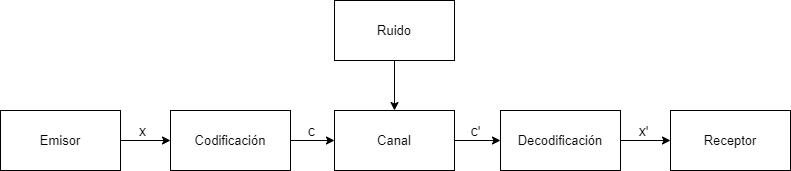
\includegraphics[scale=0.5]{figures/Diagrama_comunicacion.png}
	\caption{Esquema del modelo de comunicación, \cite{Podesta_2006}.}
\end{figure}

Las flechas indican que la comunicación es en un solo sentido.

En general, $x' \neq x$ y es deseable que este error sea detectado (lo cual permite pedir una retransmisión del mensaje) y en lo posible corregido.

La \emph{Teoría de Códigos Autocorrectores} se ocupa del segundo y cuarto pasos del esquema anterior, es decir, de la codificación y decodificación de mensajes, junto con el problema de detectar y corregir errores. A veces no es posible pedir retransmisión de mensajes y es por eso que los códigos autocorrectores son tan útiles y necesarios.

La calidad de un código con mensajes de longitud $k$ y palabras código de longitud $n$ vendrá dada por las siguientes características.

\begin{itemize}
    \item El cociente $\frac{k}{n}$, el \emph{ratio de información} del código, que mide el esfuerzo necesario para transmitir un mensaje codificado.
    \item La \emph{distancia mínima relativa} $d$ que es aproximadamente el doble de la proporción de errores que se pueden corregir en cada mensaje codificado.
    \item La \emph{complejidad} de los procedimientos de codificar y decodificar.
\end{itemize}

De esta forma, uno de los objetivos centrales de la teoría de códigos autocorrectores es construir códigos que sean de calidad. Esto es, códigos que permitan codificar muchos mensajes, que se puedan trasmitir rápida y eficientemente, que detecten y corrijan simultáneamente la mayor cantidad de errores posibles y que haya algoritmos de decodificación eficientes y efectivos. Por lo que habrá que encontrar un balance entre estas distintas metas, pues suelen ser contradictorias entre sí.

\spacedlowsmallcaps{Descripción del trabajo}

El objetivo principal de este trabajo se basa en emplear algoritmos genéticos para realizar un análisis del criptosistema de McEliece clásico. En consecuencia, haremos uso de las técnicas y áreas de las matemáticas, tales como los cuerpos finitos, los anillos de polinomios sobre cuerpos finitos y la complejidad de los problemas y de los algoritmos. En cuanto a las herramientas informáticas, hablaremos de las metaheurísticas basadas en poblaciones, en concreto los algoritmos genéticos. A lo largo del desarrollo de este trabajo, ilustraremos en los ejemplos las implementaciones realizadas en el sistema algebraico computacional SageMath.

\spacedlowsmallcaps{Contenido del trabajo}

El contenido de este trabajo comienza con un capítulo dedicado a describir y desarrollar las herramientas matemáticas e informáticas que necesitaremos para facilitar el seguimiento del posterior desarrollo. Estudiaremos los conceptos básicos relacionados con la teoría de códigos lineales, que nos permitirá introducir las bases para que en el siguiente capítulo podamos desarrollar los códigos de Goppa. A partir de estos códigos, podremos construir el criptosistema de McEliece clásico y emplear los algoritmos genéticos para concluir con su respectivo análisis.

\spacedlowsmallcaps{Objetivos del trabajo}

Los objetivos de este trabajo son los siguientes.

\begin{itemize}
    \item Estudiar la teoría básica de códigos lineales.
    \item Estudiar los códigos de Goppa y su decodificación.
    \item Estudiar la criptografía basada en códigos como modelo de criptografía post-cuántica.
    \item Estudiar e implementar el criptosistema de McEliece.
    \item Estudiar e implementar algoritmos evolutivos para el cálculo de la distancia de un código lineal.
    \item Estudiar el criptoanálisis del criptosistema de McEliece mediante algoritmos evolutivos.
\end{itemize}